%%%%%%%%%%%%%%%%%%%%%%%%%%%%%%%%%%%%%%%%%
% Academic Title Page
% LaTeX Template
% Version 2.0 (17/7/17)
%
% This template was downloaded from:
% http://www.LaTeXTemplates.com
%
% Original author:
% WikiBooks (LaTeX - Title Creation) with modifications by:
% Vel (vel@latextemplates.com)
%
% License:
% CC BY-NC-SA 3.0 (http://creativecommons.org/licenses/by-nc-sa/3.0/)
% 
% Instructions for using this template:
% This title page is capable of being compiled as is. This is not useful for 
% including it in another document. To do this, you have two options: 
%
% 1) Copy/paste everything between \begin{document} and \end{document} 
% starting at \begin{titlepage} and paste this into another LaTeX file where you 
% want your title page.
% OR
% 2) Remove everything outside the \begin{titlepage} and \end{titlepage}, rename
% this file and move it to the same directory as the LaTeX file you wish to add it to. 
% Then add \input{./<new filename>.tex} to your LaTeX file where you want your
% title page.
%
%%%%%%%%%%%%%%%%%%%%%%%%%%%%%%%%%%%%%%%%%

%----------------------------------------------------------------------------------------
%	PACKAGES AND OTHER DOCUMENT CONFIGURATIONS
%----------------------------------------------------------------------------------------

\documentclass[11pt]{article}

\usepackage[italian]{babel}

\usepackage[utf8]{inputenc} % Required for inputting international characters
\usepackage[T1]{fontenc} % Output font encoding for international characters

\usepackage{mathpazo} % Palatino font
\usepackage{graphicx}
\usepackage{fancyhdr}
\usepackage{tabularx}
\usepackage{geometry}

\geometry{legalpaper, margin=2.5cm}

\newcommand{\doctitle}{Impact Analysis Report}
\newcommand{\docversion}{1.0}

\begin{document}
	
	%----------------------------------------------------------------------------------------
	%	TITLE PAGE
	%----------------------------------------------------------------------------------------
	
	\begin{titlepage} % Suppresses displaying the page number on the title page and the subsequent page counts as page 1
		\newcommand{\HRule}{\rule{\linewidth}{0.5mm}} % Defines a new command for horizontal lines, change thickness here
		
		\center % Centre everything on the page
		
		%------------------------------------------------
		%	Headings
		%------------------------------------------------
		
		\textsc{\LARGE Università degli Studi di Salerno}\\
		\textsc{\large Corso di Ingegneria del Software}\\[1.5cm] % Main heading such as the name of your university/college
		
		%------------------------------------------------
		%	Title
		%------------------------------------------------
		
		\HRule\\[0.4cm]
		
		{\huge\bfseries ASCETIC}\\ % Title of your document
		\vspace{0.2cm}
		{\large\bfseries Automated Code Smell Identification and Correction}\\[0.2cm] % Title of your document
		
		\HRule\\[1.5cm]
		
		\textsc{\Large \doctitle}\\[0.3cm] % Major heading such as course name
		
		\textsc{\large Version \docversion}\\[0.5cm] % Minor heading such as course title
		
		
		%------------------------------------------------
		%	Logo
		%------------------------------------------------
		
		\vfill\vfill
		
		
\includegraphics[width=0.5\textwidth]{../logo_temp.jpg}\\[1cm] % Include a department/university logo - this will require the graphicx package
		
		%------------------------------------------------
		%	Date
		%------------------------------------------------
		
		\vfill\vfill\vfill % Position the date 3/4 down the remaining page
		
		{\large\today} % Date, change the \today to a set date if you want to be precise
		
	
		
		%----------------------------------------------------------------------------------------
		
		\vfill % Push the date up 1/4 of the remaining page
		
	\end{titlepage}
	
	%----------------------------------------------------------------------------------------
	
	\pagestyle{fancy}
	\rhead{ASCETIC}
	\lhead{\doctitle~v.~\docversion}
	\renewcommand{\headrulewidth}{0pt}
	
	
	\textbf{Coordinatore Progetto:}
	\begin{table}[h]
		\centering
		\begin{tabularx}{0.9\textwidth}{|X|X|}
			\hline
			\textbf{Nome}     & \textbf{Matricola} \\ \hline
			Manuel De Stefano &  0522500633\\ \hline
		\end{tabularx}
	\end{table}

	\vspace{0.5cm}
	
	\textbf{Partecipanti:}
	\begin{table}[h]
		\centering
		\begin{tabularx}{0.9\textwidth}{|X|X|}
			\hline
			\textbf{Nome}     & \textbf{Matricola} \\ \hline
			Amoriello Nicola &  0512104742\\ \hline
			Di Dario Dario &  0512104758\\ \hline
			Gambardella Michele Simone &  0512104502\\ \hline
			Iovane Francesco &  0512104550\\ \hline
			Pascucci Domenico &  0512102950\\ \hline
			Patierno Sara &  0512103460\\ \hline
		\end{tabularx}
	\end{table}

	\textbf{Revision History:}
	\begin{table}[h]
		\centering
		\begin{tabularx}{0.9\textwidth}{|p{2cm}|l|p{2cm}|X|p{2cm}|}
			\hline
			\textbf{Data} & \textbf{Versione}& \textbf{C.R. Interessata} & \textbf{Descrizione} & \textbf{Autore} \\ \hline
			24/10/2018 & 1.0 & CR3 & Prima Stesura & Manuel De Stefano \\ \hline
		\end{tabularx}
	\end{table}

	\vfill
	\newpage
	
	\tableofcontents
	\newpage
	
	\section{Introduzione}
		In questo documento verrà analizzato l'effetto che la \textbf{Change Request n$^\circ$3} avrà sul sistema. 
		
		\paragraph{} \textbf{La Change Request n$^\circ$3} ha come scopo la modifica, o meglio, il \textit{refactoring} di alcuni sottosistemi con l'obiettivo di favorirne il riuso, la manutenzione e l'evoluzione. Nella change request viene suggerito l'applicazione di \textbf{\textit{Design Patterns}} specifici e l'uso di particolari astrazioni, proprio per poter raggiungere lo scopo.
		
		\paragraph{} In questo documento verrà riportata l'analisi fatta sul codice e le modifiche ad esso riportate, verificandone la fattibilità e l'impatto su altre componenti codice. I risultati di queste modifiche verranno riportati, oltre che in questo documento, anche nel documento di \textbf{Object Design}.
	

	\section{Identificazione degli Impact Set}
	
	\subsection{Starting Impact Set}
	L'identificazione dello \textbf{starting impact set} è stata particolarmente semplice, in quanto il testo della change request riportava esplicitamente i moduli su cui effettuare le modifiche: il package \textit{\textbf{Parser}}, il package \textbf{\textit{CodeSmellDetection}} e il package \textit{\textbf{Refactoring}}, compresi delle classi in essi contenuti. Lo \textit{starting impact set}, dunque, comprende i seguenti componenti: 
	
	\begin{itemize}
		\item Package \textbf{Parser}, contenente le seguenti classi:
			\begin{itemize}
				\item BeanConverter
				\item PackageParser
				\item ClassPaerser
				\item MethodParser
				\item InstanceVariableParser
			\end{itemize}
		
		\item Package \textbf{CodeSmellDetection}, contenente le seguenti classi:
			\begin{itemize}
				
				\item BlobRule
				\item FeatureEnvyRule
				\item MisplacedClassRule
				\item MisplacedComponentsUtilities
				\item PromiscuousPackageRule
				\item ComponentMutation
				\item StructuralFeatureEnvyRule
				\item StructuralMisplacedClassRule
							
			\end{itemize}
		
		\item Package \textbf{Refactoring}, contenente le seguenti classi:
		
			\begin{itemize}
				
				\item RefactorManager
				\item MoveMethodRefactoring
				\item SearchUtil
						
			\end{itemize}	
			
		
		
	\end{itemize}


	\subsection{Candidate Impact Set}

	L'identificazione del \textbf{Candidate Impact Set} delle componenti codice è stata effettuata tramite l'utilizzo di (due) tools di analisi statica messi a disposizione dall'IDE Intellij IDEA. Il primo è la DSM, acronimo per \textbf{Dependency Structure Matrix}, ovvero, un metodo per esplorare dipendenze tra parti di programma (moduli, classi, ecc.) e fornire una rappresentazione matriciale compatta del progetto \cite{dsm}.
	Consente di visualizzare le dipendenze tra le parti di un progetto e di evidenziare il flusso di informazioni in un progetto.
	
	\paragraph{} Quando è pronta, la DSM View è aperta in una finestra, e consente di esaminare le dipendenze. Gli \textbf{indici di riga} rappresentano la struttura del programma. Gli \textbf{indici di colonna} sono gli stessi dei corrispondenti indici di riga. La riga selezionata e la colonna corrispondente sono evidenziate per visualizzare le dipendenze. La colonna mostra le dipendenze \textbf{della} componente che è indice di riga (cioè quelle \textbf{da cui dipende} la componente selezionata), mentre la riga mostra le dipendenze \textbf{verso} la riga selezionata (ovvero le componenti che \textbf{dipendono da quella selezionata}) \cite{dsm}. 
	
	\paragraph{}
	Queste ultime sono di particolare importanza per la nostra analisi, poiché, indicano componenti che possono essere impattate da una modifica fatta ad una componente da cui dipendono. Dunque, nel \textbf{candidate impact set} sono state inserite tutte le componenti che la DSM ha indicato come \textbf{direttamente dipendenti} dalle componenti presenti nello \textbf{starting impact set}. Nel nostro caso, andremo, dunque, a considerare le dipendenze verso i package \textbf{parser}, \textbf{CodeSmellDetection} e \textbf{Refactoring}.
	
	\subsubsection{Componenti dipendenti dal package Parser}

	Dalla \figurename~\ref{dsm1} si evincono le componenti che dipendono dal package \textbf{Parser}. Analizzando la \textbf{DSM} si può notare che le componenti che dipendono dal package in analisi sono due: il package \textbf{Actions} (con 3 dipendenze), ed il package \textbf{ProjectAnalysis} (con 1 dipendenza).
	
	\begin{figure}[h!]
		\centering
		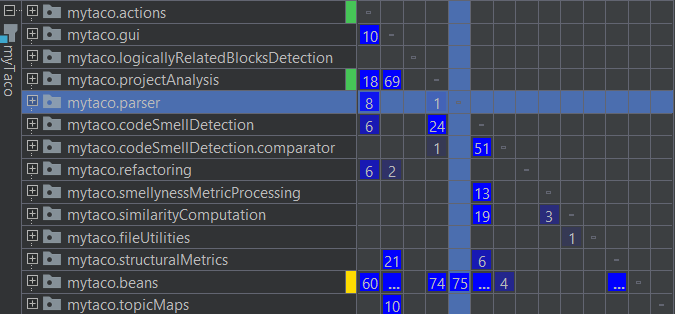
\includegraphics[width=0.8\textwidth]{dsm2.png}\\[1cm]
		\caption{DSM del package Parser}
		\label{dsm1}
	\end{figure}


	Approfondendo l'analisi delle dipendenze per il package Actions, notiamo esse siano tutte legate ad un'unica classe del package Parser, ovvero la classe \textbf{\textit{BeanConverter}}. Ciò comporta che solo una modifica a tale classe potrebbe impattare sulle classi presenti nel package Actions.
	
	\begin{figure}[h!]
		\centering
		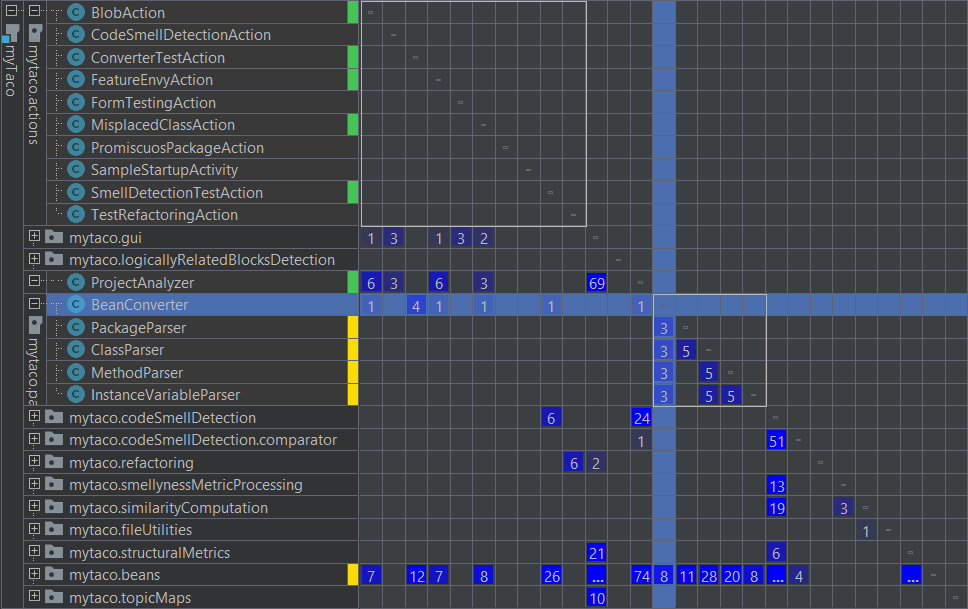
\includegraphics[width=0.8\textwidth]{dsm1.png}\\[1cm]
		\caption{DSM del package Parser}
		\label{dsm2}
	\end{figure}

	La \figurename~\ref{dsm2} mostra nel dettaglio quali classi dipendono dalla classe \textit{BeanConerter}. Nella fattispecie:
	
	\begin{itemize}
		
		\item BlobAction (1 dipendenza)
		
		\item FeatureEnvyAction (1 dipendenza)
		
		\item MisplacedClassAction (1 dipendenza)
		
		\item ProjectAnalyzer (1 dipendenza)

		
	\end{itemize}
	
	Dunque queste classi saranno inserite nel \textbf{Candidate Impact Set}.
	
	\subsubsection{Componenti dipendenti dal package CodeSmellDetection}
	
	\begin{figure}[h!]
		\centering
		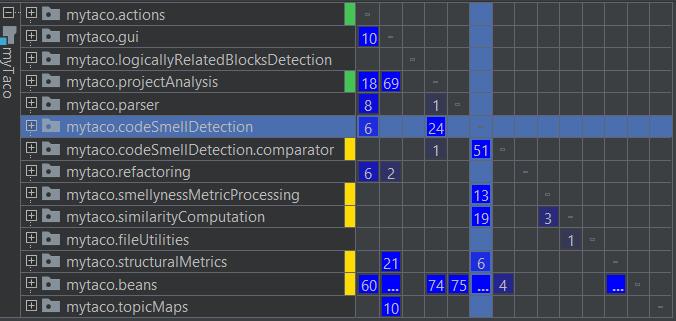
\includegraphics[width=0.8\textwidth]{dsm3.png}\\[1cm]
		\caption{DSM del package Parser}
		\label{dsm3}
	\end{figure}
	
	\subsubsection{Componenti dipendenti dal package Refactoring}
	
	
	
	\paragraph{} Il secondo tool utilizzato è lo strumento di \textbf{Data Flow Analysis}, che permette di analizzare il flusso dati \textbf{da} o \textbf{verso} il simbolo selezionato, che può essere un'espressione, una variabile o un metodo. L'output presenta una traccia di nodi che corrispondono a catene di assegnamento o invocazioni di metodi, entranti o uscenti al simbolo selezionato, a seconda dal tipo di analisi richiesta. Nel nostro caso, è stato utile analizzare il flusso dati uscente dai vari metodi delle classi presenti nello \textbf{starting impact set}, in modo da raffinare l'insieme calcolato precedentemente tramite la DSM.
	
	\section{Analisi Post-Modifica e Calcolo di Metriche}
	
	\newpage
	
	\begin{thebibliography}{9}
		
		\bibitem{dsm} Maria Khalusova. "IntelliJ IDEA: Dependency Analysis with DSM".
		\textit{Intellij IDEA Blog}. Jet Brains s.r.o, 2008. Web. Consultato il 7 Novembre 2018.
		
		\bibitem{dataflow} CDR. "Analyzing Dataflow with IntelliJ IDEA".
		\textit{Intellij IDEA Blog}. Jet Brains s.r.o, 2009. Web. Consultato il 7 Novembre 2018.
	\end{thebibliography}
	
	
\end{document}
